\documentclass[aspectratio=169,
				xcolor=table]{beamer}

% Load general definitions
\usepackage[utf8]{inputenc}
%\usepackage[T1]{fontenc}
\usepackage[brazil]{babel}
\usepackage{amsmath}
\usepackage{amsfonts}
\usepackage{amssymb}
\usepackage{graphicx}
\usepackage{verbatim}
\usepackage{cancel}
\usepackage{askmaps}
\usepackage{tabularx}
\usepackage[table]{xcolor}
%\usepackage{tikz}
\usepackage{multirow}
\usepackage{mathtools}
\usepackage{color, colortbl}
\usepackage{etoolbox}
\usepackage{pbox}
\usepackage{changepage}
\usepackage{xpatch}
\usepackage{array}
\usepackage{marvosym}
\usepackage{tabu}
\usepackage{multicol}
\usepackage{listings}
\usepackage{underscore}
\usepackage{filecontents}
\usepackage[]{algorithm2e}
\usepackage{ragged2e}

\newcolumntype{P}[1]{>{\centering\arraybackslash}m{#1}}
\definecolor{Gray}{gray}{0.75}
\definecolor{Gray2}{gray}{0.85}

\definecolor{lightBlue}{HTML}{DAE8FC}
\definecolor{Blue}{RGB}{51, 51, 204}

%\useinnertheme[lily]{rounded}
\usetheme{UniEvangelica}
%\usetheme{Copenhagen}
%\usetheme{Berlin}
%\usecolortheme{dolphin}
\tolerance=1
\emergencystretch=\maxdimen
\hyphenpenalty=10000
\hbadness=10000

\setbeamertemplate{navigation symbols}{}%remove navigation symbols


\let\olditem=\item% 
\renewcommand{\item}{\olditem \justifying}%
\def\center{\trivlist \centering\item\relax}
\def\endcenter{\endtrivlist}

\setbeamertemplate{itemize/enumerate body begin}{\large}
\setbeamertemplate{itemize/enumerate subbody begin}{\large}

\setbeamertemplate{itemize item}{\raisebox{0.1ex}{$\blacktriangleright$}\hskip0.1em}
\setbeamertemplate{itemize subitem}{\raisebox{0.1ex}{$\blacktriangleright$}\hskip0.1em}

\newcommand{\greenarrow}{\textcolor{green}{\rotatebox[origin=c]{180}{\MVArrowDown}}}

\newcommand{\redarrow}{\textcolor{red}{\MVArrowDown}}

%\newcommand{\ftable}{
%	\begin{table}
%		\large
%		\centering
%		\rowcolors{1}{\ifnumless{\rownum}{2}{Blue}{lightBlue}}{}
%}

\newenvironment{eftable}{
	\begin{table}
		\large
		\centering
		\rowcolors{1}{}{Blue}
		\rowcolors{1}{\ifnumless{\rownum}{2}{Blue}{lightBlue}}{}
	}
	{
	\end{table}
}


%\setbeamertemplate{frametitle}
%{
%	%\vspace*{-2em}	
%	\insertframetitle
%
%	 %\textcolor{white}{\LARGE \insertframetitle}
%
%}

% Specific definitions
\institute[]{\uppercase{Engenharia de Software}}
\title[]{Sistemas Operacionais}
\subtitle[]{Gerenciamento de Arquivos}
\author[]{Prof. M.e Alexandre Tannus}
\date{Anápolis - 2021.1}

\AtBeginSection{\frame{\tableofcontents[currentsection]}}
\begin{document}
	
	\begin{frame}
		\titlepage
	\end{frame}

	\begin{frame}
		\tableofcontents
	\end{frame}		
	
	
	\section{Introdução}
	\begin{frame}{Visão do Usuário Comum}
		\begin{figure}[hbtp]
			\centering
			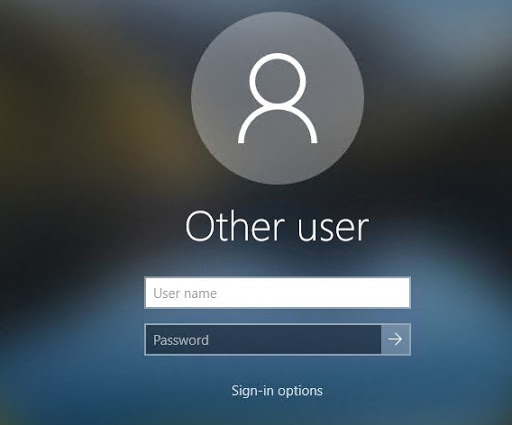
\includegraphics[height=.5\paperheight]{../figs/cap09/login.jpg}
		\end{figure}
		
	\end{frame}
	
	
	\begin{frame}{Visão do Usuário Comum}
		\begin{figure}[hbtp]
			\centering
			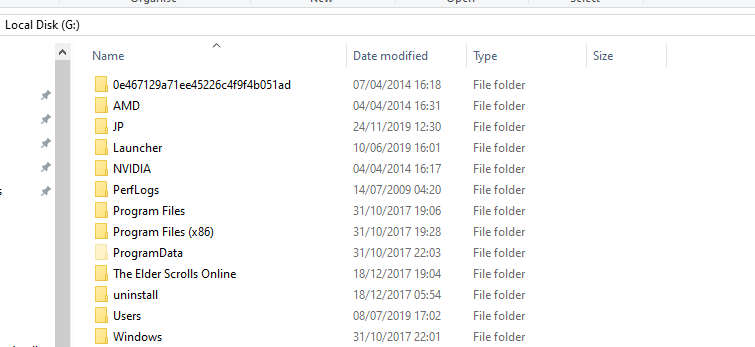
\includegraphics[height=.7\paperheight]{../figs/cap09/structure.png}
		\end{figure}		
	\end{frame}
	
	\begin{frame}{Introdução}
		\begin{itemize}
			\item Armazenamento e recuperação de informação são essenciais
			\vspace{1em}
			\item Requisitos fundamentais
			\begin{itemize}
				\item Armazenamento de grande volume de informações
				\item Manutenção dos dados após finalização do processo
				\item Acesso concorrente
			\end{itemize}
			\vspace{2em}
			\item \alert{Solução:} \textbf{Armazenamento em discos ou outras mídias externas de forma persistente}			
			
		\end{itemize}
	\end{frame}
	
	\begin{frame}{Persistência de arquivos}
		\begin{itemize}
			\item Informações devem ser armazenadas em \textbf{arquivos}
			\begin{itemize}
				\item Não devem ser afetadas por criação ou término de processos
				\item O arquivo só pode desaparecer quando seu criador o remover
			\end{itemize}
			\vspace{1.5em}
			\item Sistema de arquivos
			\begin{itemize}
				\item Parte do sistema operacional que gerencia os arquivos
			\end{itemize}
		\end{itemize}
		
	\end{frame}
	\begin{frame}{Sistema de arquivos - Aspectos importantes}
		\begin{itemize}
			\item Usuário
			\begin{itemize}
				\item Nomenclatura
				\item Proteção
				\item Operações permitidas
			\end{itemize}
			\vspace{1em}
			\item Projetistas
			\begin{itemize}
				\item Formas de implementação
				\item Alocação de espaço
			\end{itemize}
		\end{itemize}
		
	\end{frame}
	
	\section{Arquivos}
	\begin{frame}{Arquivos - Definição}
		\begin{itemize}
			\item Informações logicamente relacionadas
			\begin{itemize}
				\item Representam instruções ou dados
				\item Podem possuir estrutura livre (texto) ou rígida (banco de dados relacional) 
			\end{itemize}
		\end{itemize}	
	\end{frame}
	
	\begin{frame}{Atributos dos Arquivos}
		\begin{itemize}
			\item Nome
			\vspace{1em}
			\item Identificador
			\vspace{1em}
			\item Tipo
			\vspace{1em}
			\item Locação
			\vspace{1em}
			\item Tamanho
			\vspace{1em}
			\item Proteção
		\end{itemize}
	\end{frame}
	
	\begin{frame}{Tipos de Arquivos}
		
		\begin{figure}[hbtp]
			\centering
			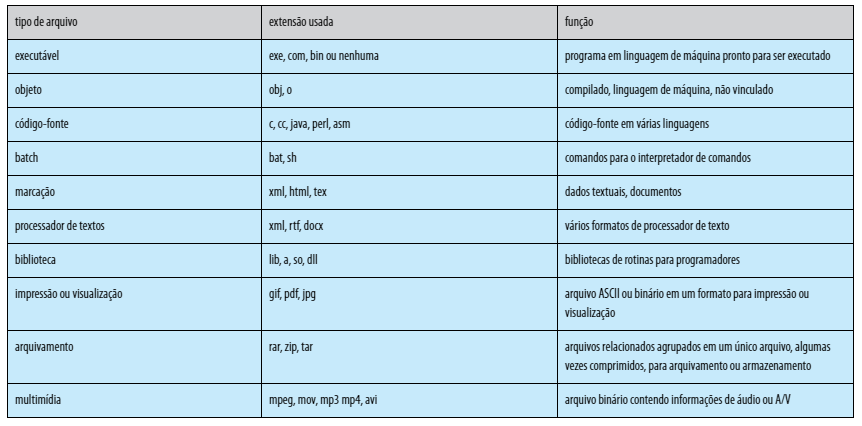
\includegraphics[height=.7\paperheight]{../figs/cap09/tipos.png}
		\end{figure}
			
	\end{frame}
	
	\begin{frame}{Operações de Arquivo }
		\begin{itemize}
			\item Criação
			\vspace{1em}
			\item Gravação
			\vspace{1em}
			\item Leitura
			\vspace{1em}
			\item Reposicionamento
			\vspace{1em}
			\item Exclusão
			\vspace{1em}
			\item Truncamento		
		\end{itemize}
	
	\end{frame}
	
	\begin{frame}{Organização de Arquivos}
		\begin{itemize}			
			\item Forma como os dados estão armazenados.
			\vspace{1em}
			\item Estruturas diferentes de acordo com o propósito
			\vspace{1em}
			\item Pode ser definida no momento da criação
		\end{itemize}
	\end{frame}
	
	\begin{frame}{Formas de Organização}
		
		\begin{figure}[hbtp]
			\centering
			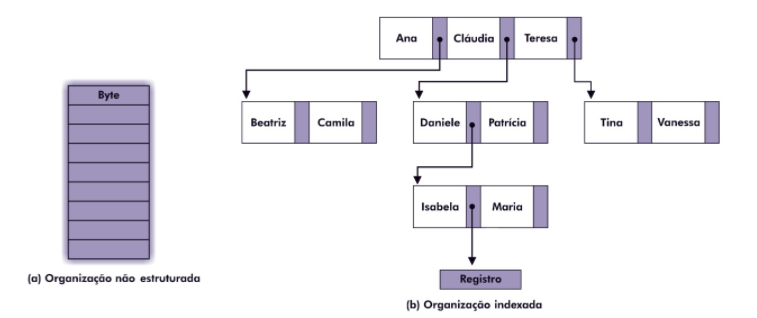
\includegraphics[height=.7\paperheight]{../figs/cap09/organizacao.png}
		\end{figure}		
	\end{frame}
	
	\begin{frame}{Métodos de Acesso}
		\begin{itemize}
			\item Formas de recuperar registros
			\begin{itemize}
				\item Sequencial
				\item Acesso Direto
				\item Acesso Indexado
			\end{itemize}
		\end{itemize}
		
	\end{frame}
	
	\section{Diretórios}
	\begin{frame}{Diretórios}
		\begin{itemize}
			\item Organização lógica dos arquivos contidos em um disco
			\vspace{1em}
			\item Contém entradas associadas aos arquivos com informações de
			\begin{itemize}
				\item Localização física
				\item Nome
				\item Organização
				\item Outros atributos
			\end{itemize}
			
		\end{itemize}
	\end{frame}
	
	\begin{frame}{Operações em diretórios}
		\begin{itemize}
			\item Busca de arquivo
			\vspace{1em}
			\item Criação de arquivo
			\vspace{1em}
			\item Exclusão de arquivo
			\vspace{1em}
			\item Renomeação de arquivo
			\vspace{1em}
			\item Listagem de diretório
			\vspace{1em}
			\item Varredura no sistema de arquivos
		\end{itemize}
		
	\end{frame}
		
	\begin{frame}{Sistemas de diretórios hierárquicos}
		
		\begin{figure}[hbtp]
			\centering
			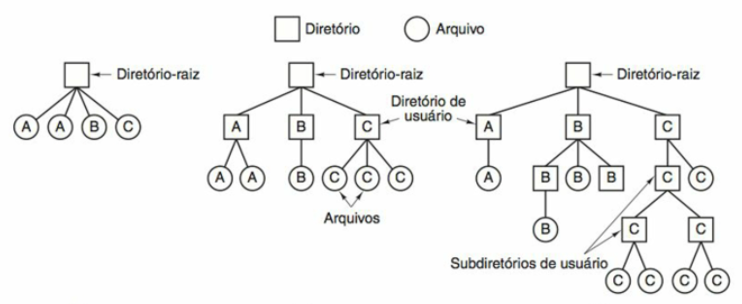
\includegraphics[height=.7\paperheight]{../figs/cap09/diretorios.png}
		\end{figure}	
	\end{frame}
	
	
	\begin{frame}{Bibliografia}
		\begin{itemize}
			\item SILBERSCHATZ, A.; GALVIN, P. B.; GAGNE, G.. \textbf{Fundamentos de sistemas operacionais: princípios básicos.} Rio de Janeiro: LTC – Livros Técnicos e Científicos, 2013.
			
			\vspace{1em}

			\item TANENBAUM, A.S., WOODHULL, A.S. \textbf{Sistemas Operacionais.} Porto Alegre: Grupo A, 2008.
			
		\end{itemize}
	\end{frame}


	\begin{frame}{}
	\end{frame}	
	
\end{document}
